\documentclass[12pt]{article}
\usepackage[utf8]{inputenc}
\usepackage{graphicx}
\usepackage[document]{ragged2e}
\renewcommand*\contentsname{Sommaire}

\begin{document}
\begin{titlepage}
\begin{center}
   \vspace*{1cm}
    \textbf{Rapport Intelligence Artificielle}
    \vspace{0.5cm}
   
    \vspace{1.5cm}
   
    \texttt{Terral Naomie}\\
    \texttt{Rodriguez Charlotte}\\
    \texttt{Geshkovski Borjan}
    \vfill
    
    \vspace{0.8cm}
    
   Université de Bordeaux\\
   Mai 2016
\end{center}
\end{titlepage}
\title{}
\tableofcontents
\clearpage

\section{Introduction à l'intelligence artificielle}

\subsection{L'intelligence artificielle en bref}
\justify
L'intelligence artificielle (IA) est un domaine de l'informatique consacré au développement de programmes, permettant aux ordinateurs d'avoir un comportement que l'on peut caractériser d'intelligent. La majeur partie de la recherche en intelligence artificielle est focalisée sur des applications extrêmement précises, telles que la prise de décision, la perception, l'adaptation à un nouvel environnement, la mémoire... 
\justify
Un des buts principaux de l'IA est de construire des entités intelligentes autonomes, capables d'exécuter des tâches complexes à la portée de l'être humain ou non. 
\justify
Dans la communauté informatique, on observe des divergences d'opinions quant aux objectifs de l'intelligence artificielle. 
\begin{itemize}
\item Doit-elle avoir seulement l'apparence de l'intelligence? (Intelligence artificielle forte)
\item Son fonctionnement interne doit-il seulement être semblable à celui de l'être humain, et être au moins aussi rationnel ? (Intelligence artificielle faible)
\end{itemize}
Dans le cadre de ce projet, nous nous situons plutôt dans le domaine de l'intelligence artificielle faible, en cherchant à reproduire le mécanisme de la prise de décision de l'être humain. 
\justify
L'intelligence artificielle s'est illustrée, au cours du temps, dans différentes applications. On a pu observer des utilisations de l'intelligence artificielle dans les jeux de stratégie (nécessitant une prise de décision). 
\justify
Un des événements les plus marquants de ces 30 dernières années, est la victoire de Deep Blue (superordinateur conçu par IBM), sur le champion du monde d'échec des années 90 Garry Kasparov. On se rappelle aussi de la victoire de Watson (aussi conçu par IBM), au jeu télévisé Jeopardy!, en 2011. Encore plus récemment, en 2015, le logiciel AlphaGo créé par Google a battu le triple champion européen de jeu de Go.
\justify
Une autre application intéressante est le développement de chatbots, comme telles qu'ELIZA, codée par Joseph Weizenbaum dans les années 60. Elle simule un dialogue actif entre un psychothérapeute (l'ordinateur) et son patient (l'utilisateur). C'est une intelligence artificielle au sens de l'intelligence artificielle faible, puisqu'elle ne comprend pas ce que l'interlocuteur lui dit, et ses réponses sont construites à partir de modèles pré-établis et de mots clés identifiés dans l'entrée de l'utilisateur.
\justify
Il y a quelques mois, Microsoft a subit un lourd échec avec la chatbot Taytweets, un compte Twitter simulant le langage d'une jeune adulte de 19 ans, dans le but d'apprendre à interagir avec les utilisateurs de ce réseaux social.
\subsection{Le problème}
\justify
Dans ce rapport nous tendons d'aborder la question de la prise de décision, élément central de l'intelligence artificielle. Nous abordons cette problématique, selon trois points de vue différents : celui d'un agent autonome, celui d'un consommateur, et celui d'une entreprise. 
\justify
Avant de poursuivre plus, définissons les notions d'agent et de prise de décision.
\justify
Un agent est "une entité autonome, capable de percevoir son environnement grâce à des capteurs, et aussi d'agir sur celui-ci via des effecteurs afin de réaliser des buts. Un agent peut également apprendre et utiliser des connaissances pour pouvoir réaliser ses objectifs"\footnote{Stuart Russel et Peter Norvige, Intelligence Artificielle, 2012}.
\justify
Dans ce projet, l'agent est un aspirateur plus ou moins intelligent (il ne disposera pas obligatoirement de capteurs). Nous étudions trois classes d'aspirateurs : 
\begin{itemize}
\item Un aspirateur aléatoire
\item Un aspirateur disposant d'une base de règle, associée à la possibilité d'apprentissage
\item Un aspirateur dit "génétique", dont le comportement est déterminé par un algorithme d'optimisation (algorithme génétique)
\end{itemize}
On entend par prise de décisions le processus qui consiste à faire un choix parmi plusieurs alternatives.
Dans le dictionnaire, une prise de décision est définie comme étant un processus cognitif complexe consistant en un choix d'actions parmi plusieurs alternatives. 
\justify
Au cours de ce travail nous nous concentrons sur la prise de décision (choix d'action entre aspiration et déplacement) de ces différents types d'aspirateurs, en fonctionne leurs capteurs et leur environnement. On regardera aussi les choix fait par les entreprises et les consommateurs. 
\section{Etudes comparative}
Le monde dans lequel les agents évoluent est un damier: il est composé de $n \times m$ cases (on note $n$ le nombre de lignes et $m$ le nombre de colonnes), dans lesquelles peut se trouver l'agent, et / ou différents objets (qui varient en fonction de l'agent considéré). L'agent se trouve forcement dans une et une seule des cases du monde.
Nous nous intéressons aux mondes unidimensionnels, l'agent ne peut donc se déplacer qu'en colonne. Dans le monde, en plus de l'unique instance d'aspirateur, se trouvent différents objets, ce qui nous ramène a faire deux études en fonction de ce contenu. Les mondes sont alors : 
\begin{itemize}
\item "petit" monde : . : rien, x : poussière. Les agents disposant de capteurs (dans notre étude) seront de capteurs [8, 2], afin de faciliter l'implémentation de la base de connaissances de l'aspirateur "Deter" (c.f. plus bas). 
\item "grand" monde : . : rien, x : poussière, p : prise électrique, j : jouet aspirable, J : jouet déplaçable. Dans ce monde, les agents ont une propriété supplémentaire : \texttt{énergie}. Les capteurs utilisés sont [6, 8, 2].
\end{itemize}
Si l'agent choisit une action impossible a effectuer, le monde ignore cette action et reste dans l'état dans lequel il était avant le choix de cette action. Par exemple, si on est dans le cas de dimension $1 \times 2$ et si l'agent se trouve dans la deuxième colonne du monde et qu'il choisit l'action \texttt{Droite}, le monde ne change pas d'état. 
\justify
Nous allons procéder à une étude purement qualitative de la performance des différents agents à partir des fonctions \texttt{getEvaluation} et \texttt{perfGlobale}. Cependant, les valeurs observées ne sont pas directement les résultats de ces fonctions: il s'agit de la moyenne de ces résultats effectuée à partir de 10 simulations (c.f. annexe). 
\subsection{Point de vue de l'agent artificiel}
\justify
\begin{itemize}
\item Aspirateur aleatoire (qu'on appelle "Stochy")
Cet agent choisit ses actions de manière aléatoire. Il ne dispose pas de capteurs (donc le monde n'est pas observable). Il est utilisable dans les deux types de mondes (c'est a dire, le "petit" et le "grand").   
\item Aspirateur base (de connaissances) forcée (qu'on appelle "Deter")
C'est un aspirateur qui dispose de capteurs lui permettant de voir les cases du monde situées a sa position et/ou a sa gauche et/ou a sa droite. Il dispose aussi d'une base de connaissances, qui constitue des règles lui dictant des actions qu'il peut effectuer en fonction des informations qu'il reçoit via ses capteurs. Cependant, il n'a pas la capacité d'apprendre, c'est a dire, de générer de nouvelles règles et mettre a jour sa base de connaissances : la base de connaissances est fixe. "Deter" va exploiter ses règles avec une probabilité qui lui est donnée (en paramètre): la probabilité d'exploitiation notée $P_e$. Dans une situation donnée, il va utiliser les règles avec une probabilité $P_e$ et choisir une action d'une manière aléatoire avec une probabilité $1-P_e$. 
\item Aspirateur apprenant (qu'on appelle "Learny")
"Learny" est identique a "Deter", a l'exception du fait qu'il peut modifier la base de connaissances, c'est à dire, qu'il dispose de la capacité d'apprendre de nouvelles règles. Au début de la simulation, la base de connaissances peut être vide ou non. De même que pour "Deter", "Learny" a une probabilité d'exploitation $P_e$. On remarque que la probabilité d'exploitation est importante pour la performance de l'aspirateur. Une valeur suffisamment grande (mais pas trop) permet une bonne performance. Par exemple, si $P_e = 0.75$, alors $\frac{3}{4}$ des fois, "Learny" utilisera ses connaissances pour effectuer une action.
\item Aspirateur génétique (qu'on appelle "Genetic")
Son comportement est totalement déterminé : soit la liste des actions qu'il doit effectuer à chaque étape de la simulation lui est explicitement donnée, soit des règles d'action lui sont données (similairement à "Deter"). La liste d'actions (ou de règles) est construite par un algorithme génétique. "Genetic" est utilisé dans le "grand" monde seulement. Pour les simulations, nous avons fix\'e la valeur de $P_e$ a $0.75$. 
\end{itemize}
\justify
Tout les aspirateurs disposent des actions suivantes: \texttt{'Gauche'} (aller à gauche), \texttt{'Droite'} (aller a droite) et \texttt{'Aspirer'}, et en fonction du contenu du monde, une action \texttt{'Repos'}.
\justify
L'intelligence des aspirateurs repose sur différentes caractéristiques : "Learny" possède d'une mémoire, c'est a dire, d'une capacité d'apprendre, les aspirateurs génétiques possèdent un "passe" leur ayant appris les meilleures règles à appliquer dans une situation donnée. Un autre aspect de l'intelligence des agents est le fait de disposer de capteurs qui les dotent d'une capacité de perception de leur environnement.
\justify
On s'intéresse à l'intelligence des différents agents, en évaluant leur prise de décision dans une situation donnée. 
A chaque fois que l'agent choisit une action, une fonction responsable de sa mise en oeuvre renvoie un score (\texttt{score\_decision}) en fonction de la pertinence de cette action. Nous considérons ici que cette performance reflète l'intelligence de l'agent. Ainsi, la performance du point de vue de l'agent (intelligence) est donnée par la fonction \texttt{getEvaluation}. Pour notre étude qualitative, on se appuie sur deux évaluations différentes:
\begin{itemize}
\item \texttt{getEvaluation} $\rightarrow$ moyenne de tout les \texttt{score\_decision} au cours de la simulation. On la note \texttt{eval\_moyenne}
\item \texttt{getEvaluation} originale qu'on note \texttt{eval\_originale}. Elle vaut (nombre de pieces nettoyées + 1)/(taille base + 1).
\end{itemize}
\justify
L'étude qualitative des agents se fait en variant la taille du monde et durée d'une simulation. Notons que lorsqu'on varie la taille, une simulation dure 2 fois la taille du monde, alors que lorsqu'on varie le nombre de simulations, la taille du monde est fixe. 
\clearpage
\justify
\textbf{Petit Monde :}
\justify
\begin{center}
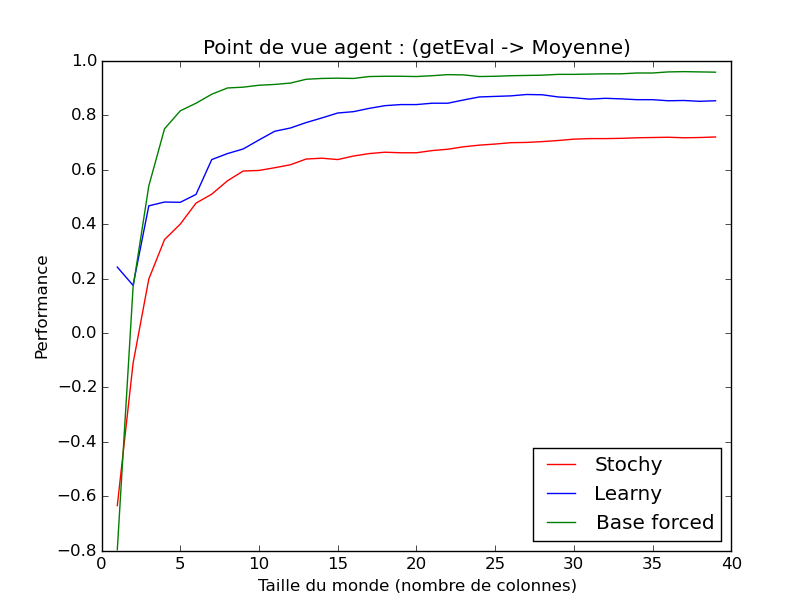
\includegraphics[scale=0.5]{geteval_moy_01}
\end{center}
\justify
En faisant varier la taille du monde, nous observons que la performance estimée par \texttt{eval\_moyenne} est la plus grande pour l'aspirateur "Deter", devant l'aspirateur "Learny" puis "Stochy". 
\begin{center}
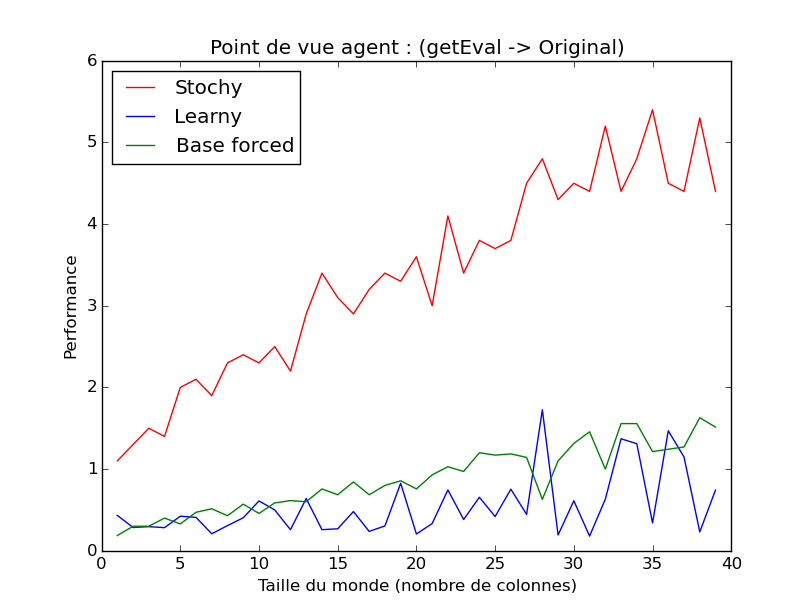
\includegraphics[scale=0.5]{geteval_orig_01}
\end{center} 
Le résultat précèdent est confirme par \texttt{eval\_orig}, mais cette évaluation n'est pas pertinente pour "Stochy", du fait de l'absence d'une base de connaissances (alors que la taille de la base de connaissances est prise en compte dans l'évaluation, et forme un biais). 
\justify
\textbf{Grand Monde :}
\begin{center}
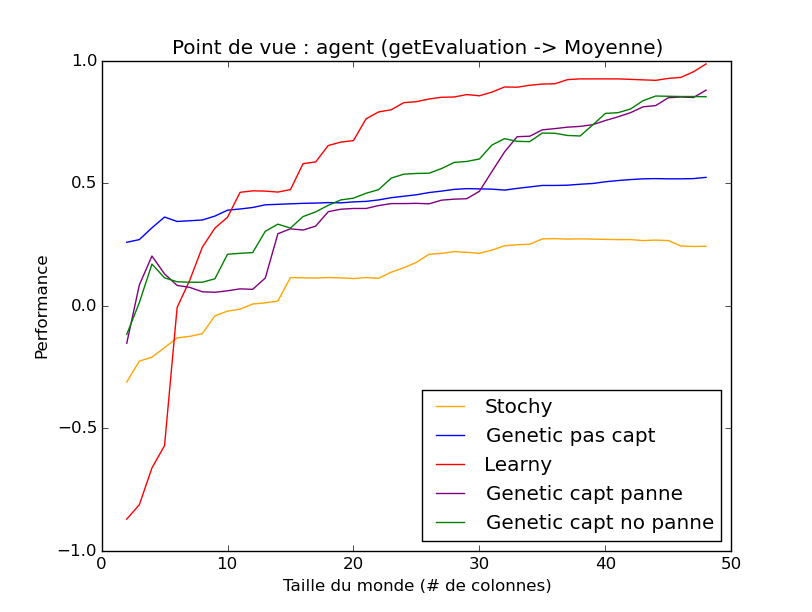
\includegraphics[scale=0.5]{geteval_moy_tout}
\end{center}
Pour l'estimation de la performance par \texttt{eval\_moyenne}, on remarque une performance croissante pour "Learny" ainsi que pour les deux aspirateurs génétiques disposant de capteurs ("Learny" en tête). Il ne semble pas y avoir de différence de performance qu'il y ait de pannes ou non (pour l'aspirateur génétique). La performance de l'aspirateur génétique sans capteurs, et de "Stochy" sont constantes.
\begin{center}
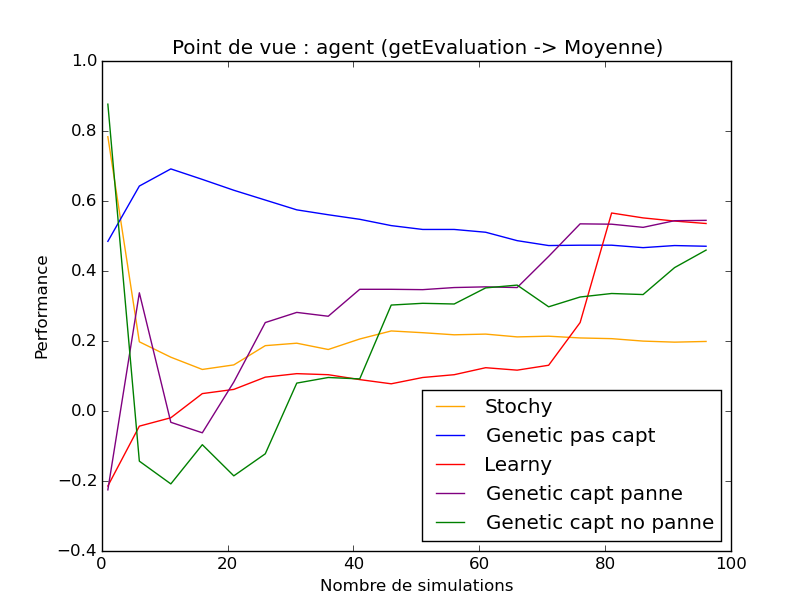
\includegraphics[scale=0.5]{simu_geteval_moy_tout}
\end{center}
\justify
On observe que la performance de "Learny", ainsi que les aspirateurs génétiques avec capteurs (sans ou avec panne) augmentent lorsque les simulations durent plus longtemps. Ceci est logique pour "Learny", puisqu'il apprend davantage.
\justify
Lorsqu'on utilise \texttt{eval\_original}, il ne semble pas y avoir une différence entre les aspirateurs, que ce soit une variation de taille du monde ou du nombre de simulations (c.f. annexe).
\justify
\textbf{Conclusion : } Dans le "petit" monde, l'aspirateur qui semble le plus intelligent est "Deter". On peut conjecturer que puisqu'il ne choisit pas ses actions aléatoirement et que la simplicité du monde permet l'implémentation d'une base de règles complète, son risque de faire un mauvais choix est très diminué. Dans un monde plus complexe, lorsque la taille de ce monde augmente, les aspirateurs qui s'adaptent le mieux semblent être "Learny" et les aspirateurs génétiques possédant les capteurs.

\subsection{Point de vue de l'entreprise commerciale}
L'entreprise utilise la fonction \texttt{perfGlobale} pour évaluer la performance de l'aspirateur. La fonction \texttt{perfGlobale} est définie de deux manières différentes en fonction du monde dans lequel se trouve l'agent : 
\begin{itemize}
\item Dans le petit monde, elle vaut nombre de pièces nettoyées - nombre de pièces visitées 3 fois ou plus.
\item Dans le grand monde, elle vaut: 
$$\frac{\mathrm{energie}}{100} + \frac{\mathrm{nettoyees}}{\mathrm{sales}} - \frac{\mathrm{nbRepos}}{\mathrm{nb \ Actions}}+\frac{\mathrm{objets \ aspirables \ apres}}{\mathrm{objets \ aspirables \ avant}} + \frac{\mathrm{nb \ tour \ vivant}}{\mathrm{nb \ tour \ max}}.$$
\end{itemize}  
\justify
\textbf{Petit Monde : }
\begin{center}
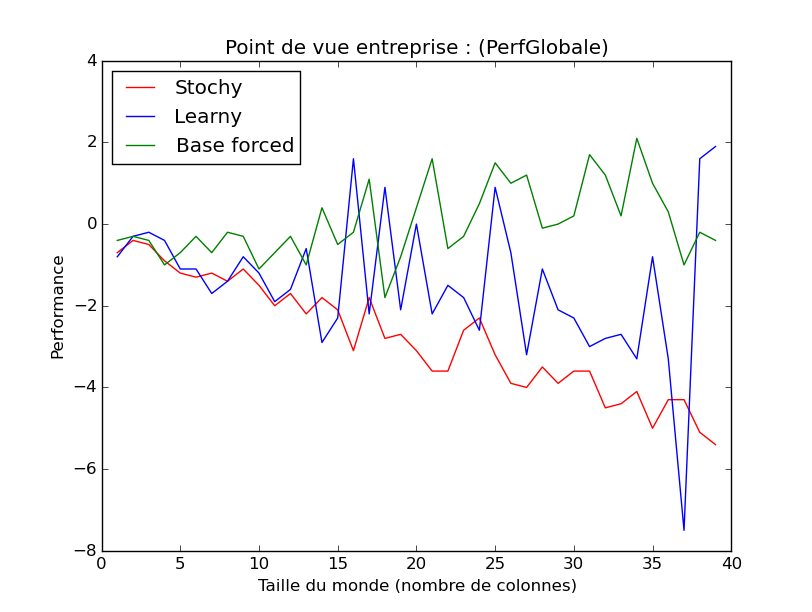
\includegraphics[scale=0.5]{perfglob_01}
\end{center}
\justify
La performance de "Stochy" est de plus en plus basse, alors que celle de "Learny" ne se stabilise pas, et n'a pas de tendance particulière. Quant a "Deter", sa performance augmente avec la taille du monde. Dans un monde qui ne contient pas d'objets, un aspirateur "Deter" à deux capteurs semble être un meilleur choix qu'un aspirateur avec une capacité d'apprentissage, d'autant plus que le monde est grand. 
\clearpage
\justify
\textbf{Grand Monde : }
\begin{center}
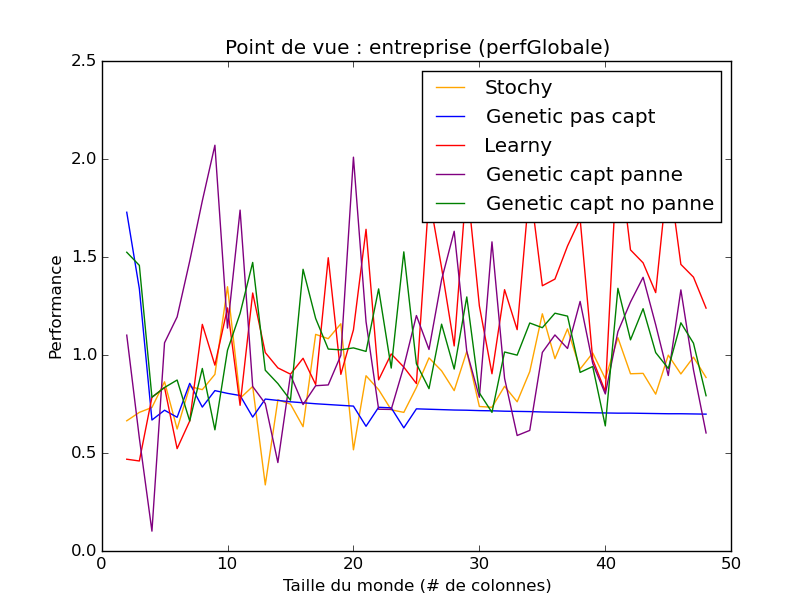
\includegraphics[scale=0.5]{perfglob_tout}
\end{center}
\justify
On remarque que l'aspirateur génétique ne possédant pas de capteurs a une performance quasi-constante lorsqu'on augmente la taille du monde. Les autres résultats ne nous apportent pas d'information pertinente.
\begin{center}
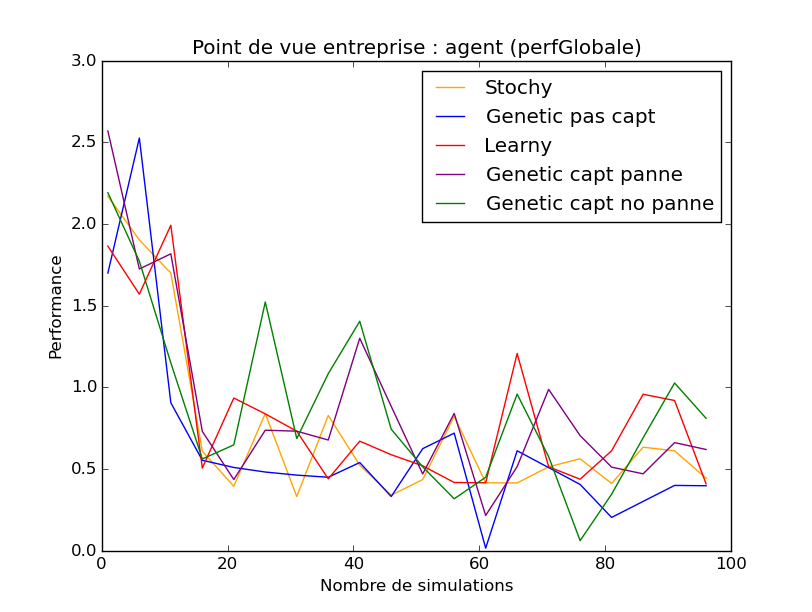
\includegraphics[scale=0.5]{simu_perfglob_tout}
\end{center}
Quant a la variation du nombre de simulations, elle nous montre que la performance diminue tres rapidement avec le nombre de simulations (jusuqu'à une durée de 20). Il ne semble pas y avoir une différence marquée entre les aspirateurs. 
\justify
Après avoir choisi, quel type d'aspirateur produire, l'entreprise doit choisir sous quelle certification il va le produire. Le tableau suivant condense les performances et les prix de fabrication en fonction des différentes certifications. Pour le rendre plus concret nous prendrons un modèle quelconque d'aspirateur, de performance 0.9 et dont la fabrication est estimée à 100 N.
\begin{center}
	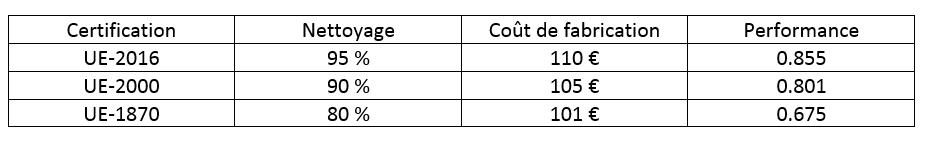
\includegraphics[scale=0.85]{Capture}
\end{center}
Ce qui signifie concrètement que pour la certification UE-1870 l'aspirateur ne nettoiera que que 80 \% de la pièce, pour un coût de production de 101 N au lieu de 100, et verra ça performance réduite à 0.675. Ainsi la certification choisie dépendra de la position de l'entreprise sur le marché.
\justify
En effet, une entreprise leader sur le marché choisira de produire son aspirateur sous la certification UE-2016. Le fait est que sa position dominante et sa réputation lui permettent de couvrir des frais de production plus élevés pour fournir un aspirateur de la meilleur qualité possible.
\justify
Alors qu'une entreprise qui n'est pas en position dominante devra faire un choix différent. En effet, elle ne pourra pas se permettre d'avoir des coûts de production trop hauts ; et malgré le faible coût d'un aspirateur certifié UE-1870, ses performances sont trop faibles pour attirer suffisamment de clients pour qu'ils s'y retrouve. Donc le meilleur choix pour ce type d'entreprise est la certification UE-2000. C'est un très bon compromis entre frais de production et performance. Le prix de production étant plus bas, l'entreprise pourra diminuer son prix de vente. Concrètement cette certification UE-2000, permet à l'entreprise de pratiquer une concurrence par les prix, avoir un produit de qualité.

\subsection{Point de vue du consommateur}
\justify
Le consommateur doit prendre deux décisions avant d'acheter un aspirateur. Il doit tout d'abord se demander quelle est la catégorie d'aspirateur la mieux adaptée à l'environnement dans lequel il doit évoluer, puis le consommateur doit choisir dans quelle entreprise il va acheter le type d'aspirateur choisi.
\justify
Le tableau suivant récapitule les compatibilités des différents aspirateurs suivant les circonstances possibles d'une pièce. 
\begin{center}
	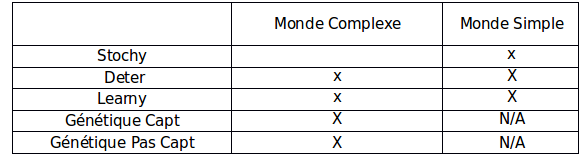
\includegraphics[scale=0.5]{2}
\end{center}
La majorité des aspirateurs (sauf Deter) sont aptes a évoluer dans un monde complexe, c'est a dire, un environnement avec des obstacles. Les aspirateurs génétique ne sont pas testés dans un monde sans obstacles (car ceci ne semble pas nécessaire, donc on ne teste pas leur performance / comportement comparativement aux autres dans ce type de monde). 
\begin{center}
	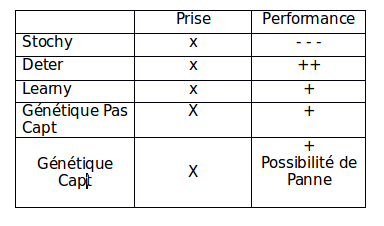
\includegraphics[scale=0.5]{3}
\end{center}
\justify
Dans un monde sans obstacles de petite taille, nous avons le choix entre les aspirateurs "Learny", "Deter" et "Stochy".
"Stochy" est peu coûteux, il aura la moins bonne performance. "Learny" peut sembler plus adaptatif, mais sa performance ne dépasse pas celle de "Deter". De plus, sa capacité d'apprentissage n'est pas exploitée de manière pertinente, donc un prix élevé pour un "accessoire" superflue ne serait pas un bon choix. "Deter" ne possède que deux capteurs, il sera donc moins cher ; ett il a la meilleure performance. Il semble être le choix le plus pertinent. Cela reste vrai lorsque la taille du monde augmente, mais les écarts de performance se creusent encore plus entre les trois aspirateurs.
\justify
Lorsque le monde est plus complexe, c'est a dire, plus variée, le consommateur a le choix entre trois types d'aspirateurs génétiques, ainsi que les aspirateurs "Learny" et "Stochy". Les aspirateurs génétiques peuvent êtres avec capteurs, ou sans capteurs, ceux possédant des capteurs coûtant plus cher. De plus, les aspirateurs génétiques avec capteurs peuvent êtres plus ou moins fiables du fait des caractéristiques de leurs capteurs. Ils peuvent ne jamais tomber en panne, ou bien, tomber en panne, de ce fait, ils peuvent coûter plus cher, ou non. A partir de cela, on peut générer l'échelle de prix suivante: Aspirateur génétique avec capteurs sans panne $>$ Aspirateur génétique avec capteur avec panne $>$ Aspirateur génétique sans capteurs $\sim$ "Learny" $>$ "Stochy". Selon son budget, le consommateur devra donc pondérer entre la qualité désirée et le prix qu'il souhaite payer. 

\justify
L'arbre de décision suivant, récapitule le meilleur choix d'aspirateur en fonction des caractéristiques de l'environnement dans lequel il devra évoluer. 
\begin{center}
	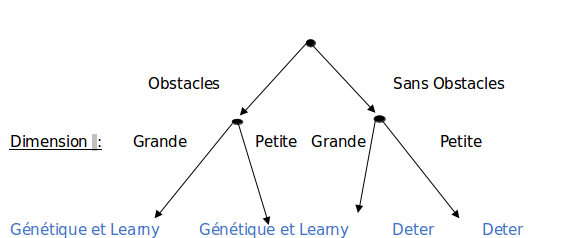
\includegraphics[scale=0.5]{1}
\end{center}
\justify
Maintenant que le consommateur sait quel type d'aspirateur autonome il lui faut, il doit maintenant choisir à quelle entreprise il va l'acheter. Il a le choix entre 3 entreprises avec des certifications différentes : Bigbro, Amzona et TombéDuCamion. Le tableau suivant condense le prix, la performance et la garantie offerts par les différentes entreprises. 
\begin{center}
	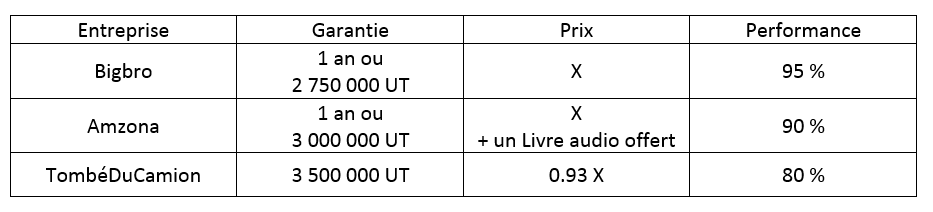
\includegraphics[scale=0.85]{ConsomEntreprise}
\end{center}
\justify
Pour pouvoir comparer les garanties, il faut savoir qu'1 an correspond à 2 592 000 UT et que lorsqu'on propose une garantie à deux composantes, dès que la première est passée, la seconde est caduque et la garantie est finie. 
\justify
Ainsi l'entreprise Bigbro propose des aspirateurs garantis 1 an ou ou 2 750 000 UT, avec une performance à 95 \% au prix de base de X N .
\justify
L'entreprise Amzona propose des aspirateurs garantis 3 000 000 UT ou 1 an, performant à 80 \% pour le même prix X N avec un livre audio offert d'une valeur de 5 \% de X N .
Pour finir l'entreprise TombéDuCamion vend des aspirateurs garantis 3 500 000 UT, avec une performance de 80 \% pour un prix équivalent à 93 \% de X. 
\justify
Globalement les performances des aspirateurs proposés par ces trois entreprises sont toutes plutôt bonnes. Mais concrètement, l'entreprise Amzona propose un aspirateur moins performant que Bigbro, pour un même prix (le cadeau est négligeable). Alors que l'entreprise TombéDuCamion propose un aspirateur un peu moins performant pour un prix inférieur aux autres, et mais avec une meilleure garantie.
\justify
Donc suivant le pouvoir d'achat du consommateur, il y a deux possibilités : 
\begin{itemize}
\item Si le consommateur a un fort pouvoir d'achat, il ira acheter son aspirateur chez Bigbro.
\item Si au contraire, le pouvoir d'achat du consommateur est plus faible, le consommateur achètera son aspirateur chez TombéDuCamion.
\end{itemize}
\clearpage
\section{Annexes}
\justify
Resultats peu significatifs : 
\begin{center}
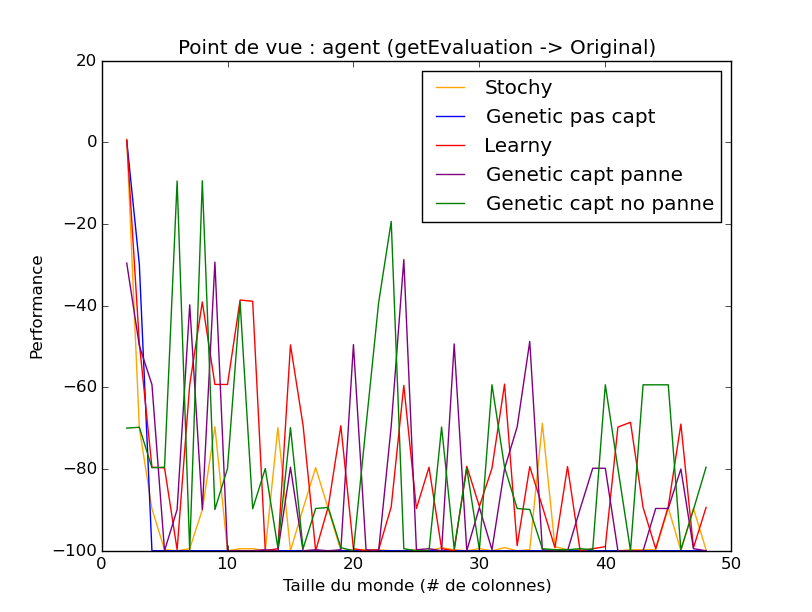
\includegraphics[scale=0.5]{geteval_orig_tout}
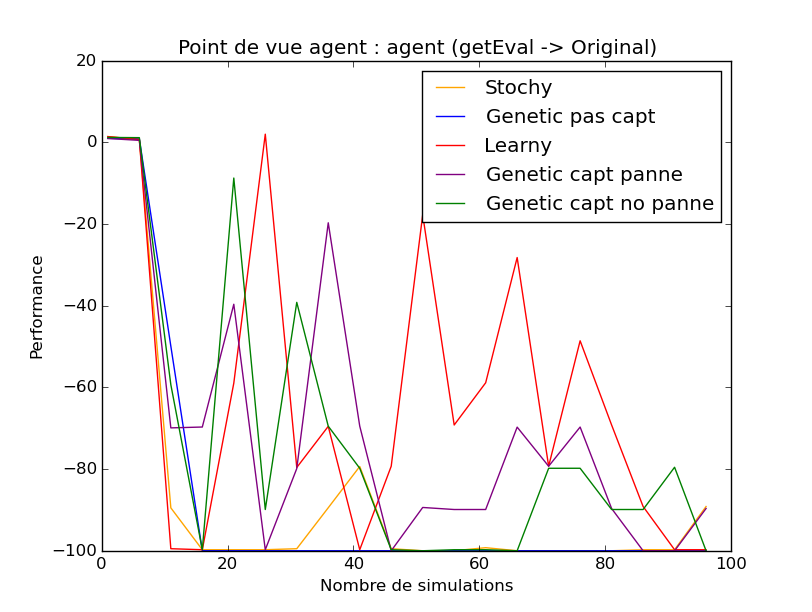
\includegraphics[scale=0.5]{simu_geteval_orig_tout}
\end{center}
\justify
Fichiers chromosome et environnement : 
\begin{itemize}
\item \texttt{\_en\_AG\_AGDR.txt} 
\item \texttt{environnements.txt}
\end{itemize}
\justify
Code utilis\'e pour les tests numeriques :
\begin{itemize}
\item "Petit" monde: \texttt{main\_tp01.py}
\item "Grand" monde: \texttt{benchmark\_aspi.py} 
\end{itemize}

\end{document}